% Hybrid fusion (proposed) — 상세판. fig_hybrid_fusion 과 Stage 1 은 같고, Stage 2 의 Patient-wise gate 와
% Cox PH combiner 를 요소 단위로 펼쳤다 (벡터 = 칸, 학습 파라미터 = 주황 칸, 연산 = 원).
%   gate:     z (2) -> C z (C 2x2, bias 없음) -> 2 sigma(.) (원소별, 범위 (0,2)) -> g (2)
%   combiner: g_m z_m -> x beta_m -> 합 -> r,  Cox PH: h(t|x) = h_0(t) e^r
%   학습:     -log PL_Efron(r) + lambda ||C||_F^2 를 beta, C 에 대해 L-BFGS 로 최소화, lambda 는 inner 4-fold CV 로 선택
% 영상 줄 y = 3.4, clinical--report 줄 y = 0 (fig_hybrid_fusion 보다 영상 줄을 올려 gate 를 두 줄 사이에 넣었다).
% 빌드: tools/build_paper_figures.sh fig_hybrid_fusion_detail
% 수치 출처: experiments/실험16_GMU_nestedCV/nested_fusion/{model.py (GatedLateFusion), config.py (GATED_LATE_LAMBDAS)}.
\documentclass[tikz,border=6pt]{standalone}
% 논문 그림 공통 스타일 (fig1/fig2 가 \input 한다).
% 시각 언어는 Mixture-of-Recursions(MoR) 논문 Fig.1/2 를 따른다:
%   파스텔 채움 + 진남색 얇은 윤곽 + 둥근 모서리, 산세리프 라벨.
% 색 의미(두 그림에서 동일):
%   boxblue   = 영상 모달리티      boxpurple = 임상 모달리티     boxpink = 판독지 모달리티
%   boxgray   = 일반 연산 블록     boxyellow = Cox 관련(head/combiner)
%   dashed    = 동결(frozen) 사전학습 모듈
\usepackage[T1]{fontenc}
\usepackage{helvet}
\renewcommand{\familydefault}{\sfdefault}
\usepackage{amsmath,amssymb}
\usetikzlibrary{positioning,arrows.meta,calc,fit,backgrounds}

\definecolor{navy}{HTML}{2F3B52}
\definecolor{ink}{HTML}{1A1A1A}
\definecolor{ink2}{HTML}{5A5E66}
\definecolor{boxblue}{HTML}{CFE0F7}
\definecolor{boxpink}{HTML}{F6CDD0}
\definecolor{boxpurple}{HTML}{DCD6F3}
\definecolor{boxyellow}{HTML}{FDEEB8}
\definecolor{boxgray}{HTML}{E9E9E9}
\definecolor{cellhold}{HTML}{3F5A8A}
\definecolor{cellfit}{HTML}{F8DD8A}
\definecolor{celleval}{HTML}{F2A4A8}

\tikzset{
  every node/.style={text=ink},
  blk/.style={draw=navy, line width=0.7pt, rounded corners=2.5pt, fill=#1,
              inner xsep=4pt, inner ysep=3pt, font=\footnotesize, align=center},
  blk/.default=boxgray,
  lay/.style={blk=#1, minimum width=30mm, minimum height=6mm},
  inp/.style={blk=#1, minimum width=15mm, minimum height=7mm},
  frozen/.style={lay=boxgray, dashed},
  container/.style={draw=navy, line width=0.8pt, rounded corners=6pt, fill=white, inner sep=6pt},
  armbox/.style={draw=navy, line width=0.6pt, dashed, rounded corners=5pt, inner sep=4pt},
  arr/.style={-{Latex[length=2.2mm,width=1.7mm]}, draw=navy, line width=0.75pt},
  lab/.style={font=\scriptsize, text=ink2, align=center, inner sep=1pt},
  op/.style={circle, draw=navy, line width=0.7pt, fill=white, inner sep=0pt,
             minimum size=4.2mm, font=\scriptsize},
  risk/.style={font=\footnotesize, inner sep=2pt},
  stage/.style={font=\scriptsize\itshape, text=ink2, inner sep=1pt},
  ptitle/.style={font=\footnotesize, align=center, inner sep=2pt},
}

% ---------------------------------------------------------------------------
% 입력 모달리티 아이콘 (fig2 입력단). 글자 라벨 대신 실제 PET-CT MIP 한 장 +
% 임상 표 / 판독지 문서 픽토그램을 쓴다. 모두 약 10.5mm x 12mm 로 크기를 맞추고
% 채움색은 모달리티 색(boxblue/boxpurple/boxpink), 윤곽은 navy 로 본문 도형과 통일.
%   사용: \iconimage{노드이름}{(x,y)}  등. 노드이름으로 화살표를 걸 수 있다.
\newcommand{\iconimage}[2]{%
  \node[blk=boxblue, inner sep=1.1pt, minimum width=0pt, minimum height=0pt] (#1) at #2
       {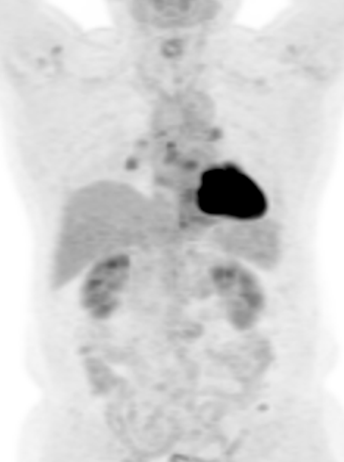
\includegraphics[height=11.8mm]{assets/pet_mip_icon.png}};%
}
\newcommand{\iconclinical}[2]{%
  \begin{scope}[shift={#2}]
    \begin{scope}
      \clip[rounded corners=2.5pt] (-5.25mm,-6mm) rectangle (5.25mm,6mm);
      \fill[boxpurple] (-5.25mm,-6mm) rectangle (5.25mm,6mm);
      \fill[navy!28]   (-5.25mm,3.3mm) rectangle (5.25mm,6mm);
      \draw[navy!45, line width=0.35pt]
        (-5.25mm,3.3mm) -- (5.25mm,3.3mm)  (-5.25mm,0.8mm) -- (5.25mm,0.8mm)
        (-5.25mm,-1.7mm) -- (5.25mm,-1.7mm) (-5.25mm,-4.2mm) -- (5.25mm,-4.2mm)
        (-1.75mm,-6mm) -- (-1.75mm,6mm)     (1.75mm,-6mm) -- (1.75mm,6mm);
    \end{scope}
    \draw[navy, line width=0.7pt, rounded corners=2.5pt] (-5.25mm,-6mm) rectangle (5.25mm,6mm);
    \node[minimum width=10.5mm, minimum height=12mm, inner sep=0pt] (#1) at (0,0) {};
  \end{scope}%
}
\newcommand{\iconreport}[2]{%
  \begin{scope}[shift={#2}]
    \fill[boxpink] (-4.6mm,-6mm) -- (-4.6mm,6mm) -- (1.7mm,6mm) -- (4.6mm,3.1mm) -- (4.6mm,-6mm) -- cycle;
    \draw[navy, line width=0.7pt, rounded corners=1pt]
      (-4.6mm,-6mm) -- (-4.6mm,6mm) -- (1.7mm,6mm) -- (4.6mm,3.1mm) -- (4.6mm,-6mm) -- cycle;
    \fill[navy!20] (1.7mm,6mm) -- (1.7mm,3.1mm) -- (4.6mm,3.1mm) -- cycle;
    \draw[navy, line width=0.55pt] (1.7mm,6mm) -- (1.7mm,3.1mm) -- (4.6mm,3.1mm);
    \draw[navy!55, line width=0.5pt]
      (-2.9mm,1.4mm) -- (2.9mm,1.4mm)  (-2.9mm,-0.4mm) -- (2.9mm,-0.4mm)
      (-2.9mm,-2.2mm) -- (2.9mm,-2.2mm) (-2.9mm,-4.0mm) -- (0.9mm,-4.0mm);
    \node[minimum width=9.2mm, minimum height=12mm, inner sep=0pt] (#1) at (0,0) {};
  \end{scope}%
}

\definecolor{learn}{HTML}{D2691E}
\colorlet{learnbg}{learn!18}
\colorlet{boxtab}{boxpurple!50!boxpink}   % clinical--report arm 의 값 (임상 + 판독지)
\newcommand{\lc}[1]{{\color{learn}#1}}   % 학습되는 값 표시
\begin{document}
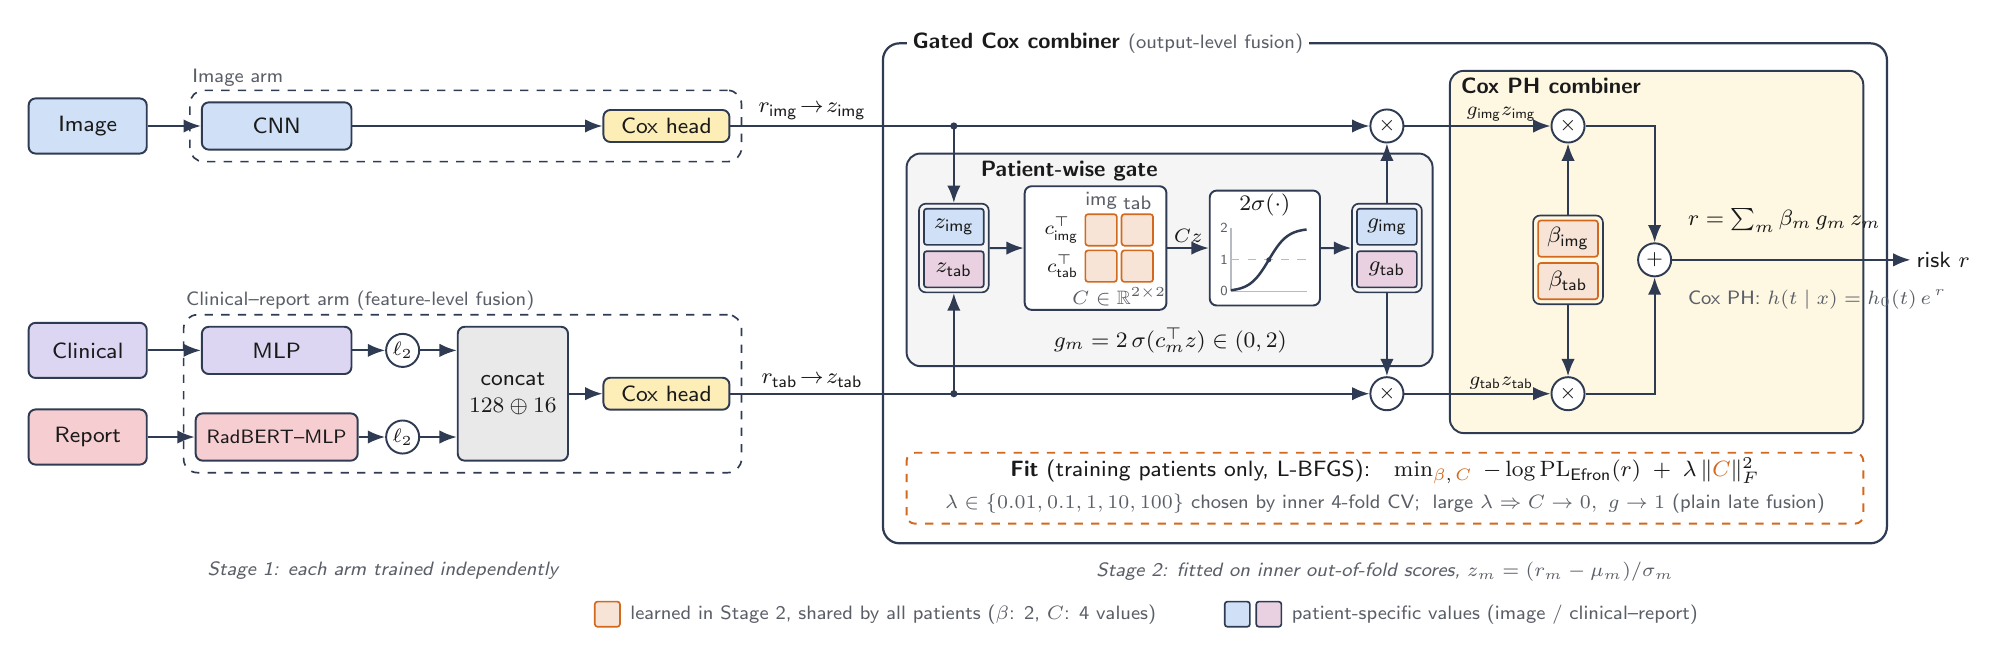
\begin{tikzpicture}[x=1cm,y=1cm,
  cell/.style={draw=navy, line width=0.6pt, rounded corners=1pt, fill=#1, minimum width=7.6mm,
               minimum height=4.6mm, inner sep=0pt, font=\footnotesize},
  pcell/.style={cell=learnbg, draw=learn},
  ccell/.style={pcell, minimum width=4mm, minimum height=4mm},
  vec/.style={draw=navy, line width=0.6pt, rounded corners=2.5pt, inner sep=1.5pt},
  sub/.style={draw=navy, line width=0.7pt, rounded corners=5pt, fill=#1},
  ttl/.style={font=\footnotesize\bfseries, inner sep=1pt},
]

% ===================== 입력 =====================
\node[inp=boxblue]   (xi) at (0,3.4)   {Image};
\node[inp=boxpurple] (xc) at (0,0.55)  {Clinical};
\node[inp=boxpink]   (xr) at (0,-0.55) {Report};

% ===================== Stage 1: 두 arm (fig_hybrid_fusion 과 같음) =====================
\node[lay=boxblue,   minimum width=19mm] (bi) at (2.4,3.4)   {CNN};
\node[blk=boxyellow, minimum width=16mm] (hi) at (7.35,3.4)  {Cox head};
\node[lay=boxpurple, minimum width=19mm] (bc) at (2.4,0.55)  {MLP};
\node[lay=boxpink,   minimum width=19mm, font=\scriptsize] (br) at (2.4,-0.55) {RadBERT--MLP};
\node[op] (lc) at (4.0,0.55)  {$\ell_2$};
\node[op] (lr) at (4.0,-0.55) {$\ell_2$};
\node[blk, minimum width=14mm, minimum height=17mm] (cat) at (5.4,0) {concat\\ $128\oplus16$};
\node[blk=boxyellow, minimum width=16mm] (ht) at (7.35,0) {Cox head};

\draw[arr] (xi) -- (bi);  \draw[arr] (xc) -- (bc);  \draw[arr] (xr) -- (br);
\draw[arr] (bc) -- (lc);  \draw[arr] (br) -- (lr);
\draw[arr] (lc.east) -- (lc.east -| cat.west);
\draw[arr] (lr.east) -- (lr.east -| cat.west);
\draw[arr] (cat) -- (ht);
\draw[arr] (bi) -- (hi);

\begin{scope}[on background layer]
  \node[armbox, fit=(bi)(hi)] (imarm) {};
  \node[armbox, fit=(bc)(br)(cat)(ht)] (tabarm) {};
\end{scope}
\node[lab, anchor=south west] at (imarm.north west)  {Image arm};
\node[lab, anchor=south west] at (tabarm.north west) {Clinical--report arm (feature-level fusion)};

% ===================== Stage 2: gated Cox combiner =====================
% 상자 (채움이 있으므로 내용보다 먼저 그린다)
\draw[container] (10.1,-1.9) rectangle (22.85,4.45);
\node[font=\footnotesize, fill=white, inner sep=2pt, anchor=west] at (10.4,4.45)
      {\textbf{Gated Cox combiner} {\scriptsize\color{ink2}(output-level fusion)}};
\draw[sub=boxgray!45]   (10.4,0.35) rectangle (17.08,3.05);
\node[ttl, anchor=north west] at (11.3,3.0) {Patient-wise gate};
\draw[sub=boxyellow!40] (17.3,-0.5) rectangle (22.55,4.1);
\node[ttl, anchor=north west] at (17.4,4.05) {Cox PH combiner};

% arm 출력 (표준화된 위험점수 z)
\node[risk, above] at (9.2,3.4) {$r_{\text{img}}\!\to\! z_{\text{img}}$};
\node[risk, above] at (9.2,0)   {$r_{\text{tab}}\!\to\! z_{\text{tab}}$};

% ---------- Patient-wise gate: z -> Cz -> 2 sigma(.) -> g ----------
% 입력 z (환자마다 다름)
\node[cell=boxblue] (zi) at (11.0,2.12) {$z_{\text{img}}$};
\node[cell=boxtab]  (zt) at (11.0,1.58) {$z_{\text{tab}}$};
\node[vec, fit=(zi)(zt)] (zv) {};
\fill[navy] (11.0,3.4) circle (1.3pt);  \fill[navy] (11.0,0) circle (1.3pt);
\draw[arr] (11.0,3.4) -- (zv.north);
\draw[arr] (11.0,0)   -- (zv.south);

% 선형 변환 C (2x2, bias 없음, 모든 환자 공통). 행 m = c_m, 열 = 곱해지는 z 성분
\node[blk=white, minimum width=18mm, minimum height=15.7mm] (cbox) at (12.8,1.85) {};
\foreach \cx in {12.87,13.33} \foreach \cy in {2.08,1.62} \node[ccell] at (\cx,\cy) {};
\node[lab, anchor=south] at (12.87,2.30) {img};
\node[lab, anchor=south] at (13.33,2.30) {tab};
\node[font=\scriptsize, anchor=east, inner sep=1pt] at (12.62,2.08) {$c_{\text{img}}^{\top}$};
\node[font=\scriptsize, anchor=east, inner sep=1pt] at (12.62,1.62) {$c_{\text{tab}}^{\top}$};
\node[lab, anchor=north] at (13.1,1.40) {$C\in\mathbb{R}^{2\times2}$};

% 2 sigma(.) : 원소별, 범위 (0,2), Cz = 0 이면 1
\node[blk=white, minimum width=14mm, minimum height=14.6mm] (sbox) at (14.95,1.85) {};
\node[font=\footnotesize, inner sep=1pt] at (14.95,2.40) {$2\sigma(\cdot)$};
\begin{scope}[shift={(15.0,1.30)}]
  \def\sx{0.12} \def\sy{0.4}
  \draw[navy!35, line width=0.4pt] ({-4*\sx},0) -- ({4*\sx},0);
  \draw[navy!35, line width=0.4pt] ({-4*\sx},0) -- ({-4*\sx},{2*\sy});
  \draw[navy!35, line width=0.4pt, dashed] ({-4*\sx},{\sy}) -- ({4*\sx},{\sy});
  \draw[navy, line width=0.9pt, domain=-4:4, samples=40, smooth] plot ({\x*\sx}, {\sy*2/(1+exp(-1*\x))});
  \fill[navy] (0,{\sy}) circle (0.9pt);
  \foreach \v in {0,1,2} \node[font=\tiny, text=ink2, anchor=east, inner sep=1pt] at ({-4*\sx},{\v*\sy}) {\v};
\end{scope}

% 출력 gate g (환자마다 다름)
\node[cell=boxblue] (gi) at (16.5,2.12) {$g_{\text{img}}$};
\node[cell=boxtab]  (gt) at (16.5,1.58) {$g_{\text{tab}}$};
\node[vec, fit=(gi)(gt)] (gv) {};

\draw[arr] (zv.east)   -- (cbox.west);
\draw[arr] (cbox.east) -- node[above, font=\scriptsize, inner sep=1.5pt] {$Cz$} (sbox.west);
\draw[arr] (sbox.east) -- (gv.west);
\node[font=\footnotesize] at (13.75,0.68) {$g_m=2\,\sigma(c_m^{\top}z)\in(0,2)$};

% ---------- gate 적용: z_m x g_m ----------
\node[op] (mgi) at (16.5,3.4) {$\times$};
\node[op] (mgt) at (16.5,0)   {$\times$};
\draw[arr] (hi) -- (mgi);
\draw[arr] (ht) -- (mgt);
\draw[arr] (gv.north) -- (mgi.south);
\draw[arr] (gv.south) -- (mgt.north);

% ---------- Cox PH combiner: x beta_m -> 합 -> r ----------
\node[op] (mbi) at (18.8,3.4) {$\times$};
\node[op] (mbt) at (18.8,0)   {$\times$};
\node[pcell] (bti) at (18.8,1.97) {$\beta_{\text{img}}$};
\node[pcell] (btt) at (18.8,1.43) {$\beta_{\text{tab}}$};
\node[vec, fit=(bti)(btt)] (bv) {};
\draw[arr] (mgi) -- (mbi);
\draw[arr] (mgt) -- (mbt);
\node[font=\scriptsize, anchor=south, inner sep=1.5pt] at (17.95,3.4) {$g_{\text{img}}z_{\text{img}}$};
\node[font=\scriptsize, anchor=south, inner sep=1.5pt] at (17.95,0)   {$g_{\text{tab}}z_{\text{tab}}$};
\draw[arr] (bv.north) -- (mbi.south);
\draw[arr] (bv.south) -- (mbt.north);

\node[op] (sm) at (19.9,1.7) {$+$};
\draw[arr] (mbi.east) -| (sm.north);
\draw[arr] (mbt.east) -| (sm.south);
\node[font=\footnotesize, anchor=west] at (20.2,2.2) {$r=\sum_m \beta_m\,g_m\,z_m$};
\node[font=\scriptsize, text=ink2, anchor=west] at (20.2,1.2) {Cox PH: $h(t\mid x)=h_0(t)\,e^{\,r}$};
\draw[arr] (sm.east) -- (23.15,1.7);
\node[risk, anchor=west] at (23.15,1.7) {risk $r$};

% ---------- 학습 (Stage 2, 학습 환자만) ----------
\draw[draw=learn, dashed, line width=0.7pt, rounded corners=3pt, fill=white] (10.4,-1.65) rectangle (22.55,-0.75);
\node[font=\footnotesize] at (16.475,-0.98)
  {\textbf{Fit} (training patients only, L-BFGS):\quad
   $\min_{\lc{\beta},\,\lc{C}}\; -\log \mathrm{PL}_{\text{Efron}}(r) \;+\; \lambda\,\lVert \lc{C}\rVert_F^2$};
\node[font=\scriptsize, text=ink2] at (16.475,-1.40)
  {$\lambda\in\{0.01,0.1,1,10,100\}$ chosen by inner 4-fold CV;\; large $\lambda \Rightarrow C\to0,\ g\to1$ (plain late fusion)};

% ===================== 단계 설명 + 범례 =====================
\node[stage, anchor=north, align=center] at (3.75,-2.1)
      {Stage 1: each arm trained independently};
\node[stage, anchor=north, align=center] at (16.475,-2.1)
      {Stage 2: fitted on inner out-of-fold scores, $z_m=(r_m-\mu_m)/\sigma_m$};

\node[pcell, minimum width=3.2mm, minimum height=3.2mm] at (6.6,-2.8) {};
\node[lab, anchor=west] at (6.85,-2.8) {learned in Stage 2, shared by all patients ($\beta$: 2, $C$: 4 values)};
\node[cell=boxblue, minimum width=3.2mm, minimum height=3.2mm] at (14.6,-2.8) {};
\node[cell=boxtab,  minimum width=3.2mm, minimum height=3.2mm] at (15.0,-2.8) {};
\node[lab, anchor=west] at (15.25,-2.8) {patient-specific values (image / clinical--report)};

\end{tikzpicture}
\end{document}
